\chapter{Introduction to Transformers}

\section{So what are transformer models and why they are taking the world by storm?}

Originally introduced in 2017 by Google researchers led by Ashish Vaswani, transformer models are a type of neural network architecture. They are designed to process sequential data (e.g., words in a sentence), such as natural language text. But here is why transformer models are revolutionary - they use a \textbf{self-attention} mechanism.\newline

This \textbf{self-attention mechanism} allows them to \textbf{focus on different parts} \textbf{of the input sequence} and \textbf{adjust} \textbf{their importance} when making predictions about the output. In contrast Recurring Neural Networks (RNNs)/ Long Short-Term Memory (LSTM)/ Gated recurrent units (GRUs) are other types of Neural Networks that process \textit{a sequence one element at a time}. Unlike self-attention, RNNs process the sequence in a linear fashion, with each element being processed sequentially based on its position in the sequence. As a result, these have a limited attention span and cannot “remember” the context from an earlier part of the sequence or conversation. Let’s see this with a visual. \newline

\href{https://www.youtube.com/watch?v=6c4bkZyztSA&ab_channel=Udacity}{Youtube} 

\subsection{Summary}

So while LSTMs have been very effective in handling sequential data, they do have some limitations:

\begin{enumerate}
    \item Limited attention span - They struggle to capture long term dependencies in sequences as they maintain a limited amount of information in memory.
    \item Computation efficiency - LSTMs are computationally expensive to train.
    \item Handling multiple sequences - LSTMs are designed to handle one sequence at a time.
\end{enumerate}
Transformers overcome all these limitations of LSTM by using \textbf{self-attention} and \textbf{parallel processing}. \newline

Transformer models have been shown to achieve state-of-the-art performance on a wide range of NLP tasks, including:

\begin{itemize}
    \item language translation
    \item text generation
    \item question answering
    \item sentiment analysis
    \item named-entity recognition
\end{itemize}
This has led to their widespread adoption in industry and academia, and they are now the dominant approach for many NLP applications. Their impact has been particularly significant in the development of large-scale language models, such as Bidirectional Encoder Representation Transformer (BERT), and Generative Pre-trained Transformer (GPT), which have revolutionized the field of NLP across a wide range of tasks.

\subsection{Open-source APIs for Transformers}

The availability of these powerful transformer models can be found in numerous open-source APIs are currently accessible from various companies, including OpenAI, TensorFlow Hub, AWS, Google Cloud AI Platform, and Hugging Face Transformers. These APIs offer convenient integration into the data pipelines of businesses, allowing them to take advantage of pre-existing transformer models in deep learning and data science. \newline

If you feel like doing a quick check on testing your understanding, do check out the quiz below.

\subsection{Quiz Question}

You are working on a natural language processing project and you are considering using a transformer model for your task. What is multi-head attention and how does it help improve the performance of a transformer model?

\begin{itemize}
    \item Multi-head attention is the ability of the transformer model to process multiple input sequences simultaneously, allowing it to handle longer sequences more effectively.
    \item \textbf{Multi-head attention is a technique for allowing the model to focus on different parts of the input sequence at different levels of abstraction, allowing it to capture more complex relationships between the words.}
    \item Multi-head attention is a mechanism for combining information from different layers of the model, allowing it to leverage information from multiple levels of abstraction.
\end{itemize}

Multi-head attention is a mechanism for allowing the model to focus on different parts of the input sequence at different levels of abstraction. This can help it capture more complex relationships between words in a sentence. It will allow the model to attend to multiple parts of the input sequence simultaneously, so multi-head attention can help it handle longer sequences more effectively.

\section{Transformers in detail}

\subsection{Transformer Architecture}
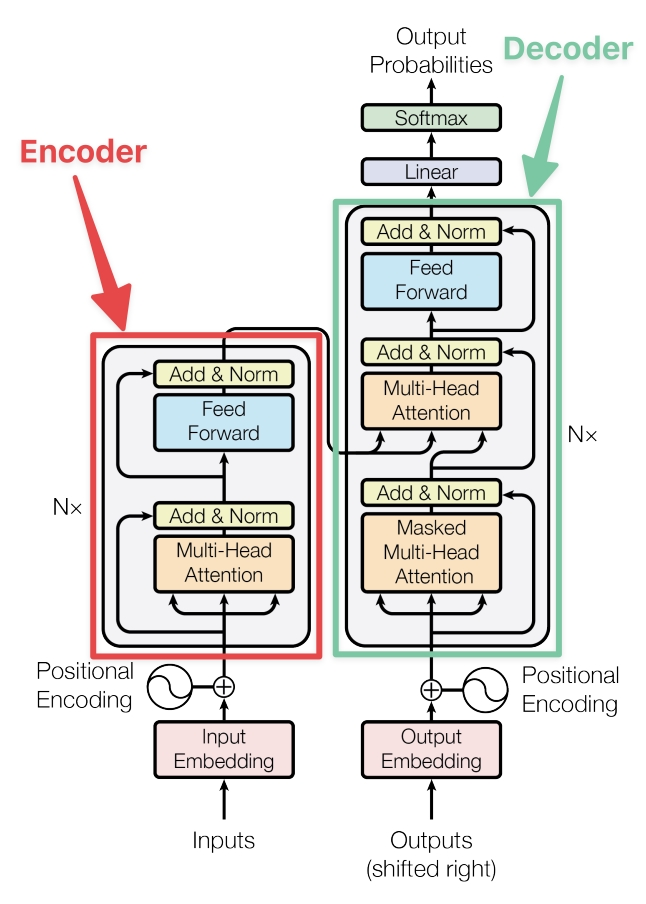
\includegraphics[width=1\linewidth]{img//rnn//transformers/transformer_architecture.jpeg}
\captionof{figure}{Transformer - model architecture [Vaswani et al. (2017). \textit{Attention is all you need.}]}

Transformers are a type of deep learning architecture that has become increasingly popular in natural language processing (NLP) tasks such as language translation and text generation. Transformers were introduced in a 2017 paper titled "Attention Is All You Need" by Vaswani et al., and have since become a cornerstone of many state-of-the-art NLP models. \newline

At a high level, the transformer architecture consists of an \textit{encoder} and a \textit{decoder}.

\begin{itemize}
    \item The encoder takes in a sequence of input tokens and produces a sequence of hidden representations
    \item The decoder takes in the encoder's output and generates a sequence of output tokens.
\end{itemize}
The key innovation of transformers is the use of \textit{self-attention} mechanisms, which allow the model to selectively focus on different parts of the input sequence when computing the hidden representations. \newline

The self-attention mechanism works by computing attention weights between each input token and all other input tokens and using these weights to compute a weighted sum of the input token embeddings. The attention weights are computed using a softmax function applied to the dot product of a \textit{query} vector, a \textit{key} vector, and a scaling factor. The query vector is derived from the previous layer's hidden representation, while the key and value vectors are derived from the input embeddings. The resulting weighted sum is fed into a multi-layer perceptron (MLP) to produce the next layer's hidden representation.\newline

More specifically, given an input sequence of length L, the encoder can be represented by a series of L identical layers, each consisting of a self-attention mechanism and a feedforward neural network:

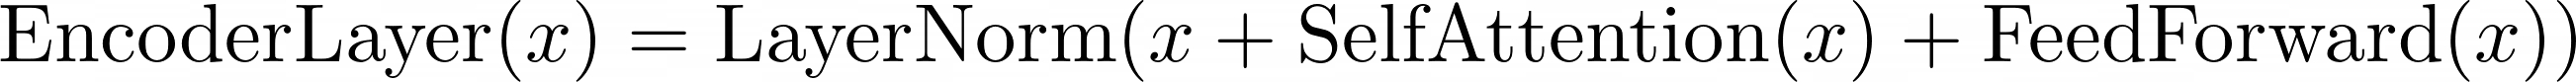
\includegraphics[width=1\linewidth]{img//rnn//transformers/eq1.jpeg}
\captionof{figure}{Encoder equation}

\href{https://www.youtube.com/watch?v=F-XN72bQiMQ&ab_channel=Udacity}{Youtube}
\subsubsection{Key, Value, and Query}

Let's try to understand \textit{the Key}, \textit{Value}, and \textit{Query} before discussing the Decoder.

The key, value, and query vectors are used in the self-attention mechanism to help the model selectively attend to different parts of the input sequence.

\begin{itemize}
    \item \textbf{Key:} You can think of the key vectors as a set of reference points the model uses to decide which parts of the input sequence are important.
    \item \textbf{Value}: The value vectors are the actual information that the model associates with each key vector.
    \item \textbf{Query}: Query vectors are used to determine how much attention to give to each key-value pair.
\end{itemize}

\begin{quote}
Example: imagine you are trying to summarize a long article. The key vectors could represent the most important sentences or phrases in the article, while the value vectors could represent the actual content of those sentences. The query vectors would then be used to decide which of these key-value pairs are most relevant to the task of summarization.

\end{quote}

The self-attention mechanism works by computing a dot product between the query vector and each key vector, which produces a set of attention weights that indicate how much attention to give to each value vector. The resulting weighted sum of the value vectors represents the attended information for that particular query.

In summary, key, value, and query vectors are used in transformers to help the model focus on important parts of the input sequence and produce more accurate and relevant output.

\subsubsection{The Mathematics behind Transformers}

The mathematics behind transformers can be quite complex, but at a high level, it involves matrix multiplications, dot products, and non-linear activations. The key equations for the self-attention mechanism can be expressed as follows:
\[Attention(Q, K, V) = softmax(\frac{QK^T}{\sqrt{d_k}})V\]
where Q, K, and V are the query, key, and value matrices, respectively, and \(d_k\) is the dimension of the key vectors. The softmax function is applied row-wise to the dot product of Q and K, which produces a set of attention weights that are used to weight the values in V. The output of the self-attention mechanism is then given by: \[MultiHead(Q, K, V) = Concat(head_1, ..., head_h)W^O\]

\subsubsection{Decoder}

The decoder is similar to the encoder but also includes an additional attention mechanism that allows it to attend to the encoder's output.

Overall, the transformer architecture has several advantages over previous NLP models. First, it is highly parallelizable, which makes it more efficient to train on modern hardware. Second, it does not rely on any explicit notion of sequence order, which allows it to better capture long-term dependencies in the input sequence. Finally, the attention mechanisms allow the model to selectively attend to different parts of the input sequence, which helps it handle tasks such as language translation where the input and output sequences may have different lengths.

\section{HuggingFace}

\begin{itemize}
    \item Hugging Face is an open-source company that provides NLP tools and models for developers and researchers. Learn more at their \href{https://huggingface.co/}{\textbf{website}}.
    \item Their flagship product is the Hugging Face Transformers library, which is a Python-based framework for building, training, and deploying state-of-the-art NLP models. Explore the library on \href{https://github.com/huggingface/transformers}{\textbf{GitHub}}
    \item Hugging Face Transformers provides pre-trained models for a variety of NLP tasks, such as text classification, question answering, machine translation, and text generation. Check out their \href{https://huggingface.co/models}{\textbf{model hub}} to browse pre-trained models.
    \item The library allows developers to quickly and easily integrate powerful NLP models into their applications using a simple API for loading pre-trained models. See the \href{https://huggingface.co/transformers/main_classes/pipelines.html}{\textbf{documentation}} for more details.
    \item The library includes a range of tools for fine-tuning models on custom datasets, making it easy to adapt models to specific tasks.
    \item Hugging Face has a large and active community that provides support, documentation, and a range of resources to help developers and researchers get the most out of the library. Join the community on their \href{https://discuss.huggingface.co/}{\textbf{forums}}.
    \item In addition to pre-trained models and tools, Hugging Face also provides datasets, evaluation metrics, and benchmarking tools for NLP. Explore their \href{https://huggingface.co/datasets}{\textbf{datasets}} and \href{https://huggingface.co/metrics}{\textbf{evaluation tools}} on their website.
    \item Hugging Face is a valuable resource for anyone working with NLP models, whether you are a developer looking to integrate models into your applications or a researcher looking to explore the state of the art in NLP. See how Hugging Face models have been used in various applications on their \href{https://huggingface.co/blog}{\textbf{blog}}.
\end{itemize}

\subsection{Benefits of using pre-trained models:}

\begin{itemize}
    \item Pre-trained models are already trained on vast amounts of data and have learned to perform well on a wide range of NLP tasks. This saves a lot of time and resources that would otherwise be spent on data collection, pre-processing, and model training.
    \item Hugging Face provides access to a large collection of pre-trained models for various NLP tasks, which are continually updated and improved. This allows developers and researchers to choose the best model for their specific use case and avoid the risk of building a suboptimal model from scratch.
    \item The Hugging Face Transformers library provides a simple API for loading and using pre-trained models, making it easy to integrate them into custom applications without requiring deep knowledge of NLP or machine learning.
\end{itemize}

\section{Benefits of Transformers}
\href{https://www.youtube.com/watch?v=lScR6pQPq9g}{Youtube} 
\subsection{Transformer Architecture Benefits}

\subsubsection{Faster to Train}
The replacement of recurrent cells with feedforward networks improves the parallelization of Transformers. Current high-performance computing systems are designed to work well with this type of parallelization.

\subsubsection{Better Performance}
Transformers offer better performance than RNNs across most natural language tasks. Therefore, we can use them to solve new problems.

\subsubsection{Versatility}
The Transformer architecture can move between different domains like NLP and Computer Vision.

\section{Intro to BERT}

\subsection{BERT Overview}

BERT (Bidirectional Encoder Representations from Transformers) is a Machine Learning (ML) model for natural language processing developed by Google in 2018. BERT is a versatile model that can handle a range of natural language processing (NLP) tasks, including but not limited to:

\begin{enumerate}
    \item Sentiment analysis
    \item Named entity recognition
    \item Question answering
    \item Language inference
    \item Text classification
    \item Paraphrasing
    \item Text summarization
    \item Machine translation
    \item Language modeling
    \item Text completion
    \item Entity linking
    \item Coreference resolution
\end{enumerate}
BERT's ability to perform well on these tasks makes it a valuable tool for many NLP applications.

\subsection{The Science Behind BERT: How it Learns and Processes Language}

To achieve its remarkable performance, BERT utilizes the following components:

\subsubsection{Extensive training data}
BERT was trained on a colossal dataset of 3.3 billion words, which is one of the main factors that contributed to its success. Specifically, it was trained on two vast datasets: Wikipedia (about 2.5 billion words) and Google's BooksCorpus (about 800 million words). By using these vast and varied datasets, BERT gained a deep understanding of natural language.

\subsubsection{MLM (Masked Language Modeling)}
MLM is a technique used by BERT to learn about the relationships between words in a sentence. In this process, BERT is trained to predict what a masked word should be based on the other words in the sentence.

\begin{quote}
\textit{Example:}

Let's say we have the following sentence: "\textit{The cat sat on the [MASK]}".

During pre-training, BERT may randomly mask one of the words in the sentence. In this case, let's say BERT masks the word "mat". The sentence would then look like this: "The cat sat on the [MASK]".

BERT is then trained to predict what the masked word should be based on the other words in the sentence. In this case, the correct answer is "mat". By considering the other words in the sentence, such as "cat" and "sat", BERT is able to make an educated guess that the missing word is "mat".

This process is repeated many times over with different sentences and different masked words, allowing BERT to learn about the relationships between words in a sentence and build a deep understanding of language.

\end{quote}

\subsubsection{NSP (Next Sentence Prediction)}
NSP is another technique used by BERT during pre-training to help it better understand the overall structure and flow of language. In this process, BERT is trained to predict whether two sentences are likely to appear together in a piece of text.

\begin{quote}
\textit{Example:}

Let's say we have two sentences:

\begin{itemize}
    \item "The cat sat on the mat."
    \item "It was a beautiful day outside."
\end{itemize}
During pre-training, BERT may be given these two sentences and asked to predict whether they are likely to appear together in a piece of text. In this case, the answer would be "no" since the two sentences do not seem to be related to each other.

BERT is trained using many different pairs of sentences, some of which are related and some of which are not. By learning to predict whether pairs of sentences are related or not, BERT gains a better understanding of the overall structure and flow of language.

This technique is important because it helps BERT understand the context in which sentences appear, which is crucial for many natural language processing tasks such as question answering and text classification.

\end{quote}

\subsection{BERT Architecture}
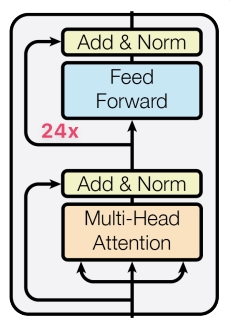
\includegraphics[width=0.5\linewidth]{bert.jpeg}
\captionof{figure}{BERTlarge - model architecture (\textit{340 million parameters})}

\begin{table}[!htbp]
\centering

\begin{tabular}{| l | l | l | l | l |}
\hline
Model & Transformer Layers & Hidden Size & Attention Heads & Parameters \\
\hline

\hline
BERTbase & 12 & 768 & 12 & 110M \\
\hline
BERTlarge & 24 & 1024 & 16 & 340M \\
\hline

\end{tabular}

\end{table}

The above table provides some key specifications of two different versions of the BERT model: \textbf{BERTbase} and \textbf{BERTlarge}.

\begin{itemize}
    \item \textbf{Transformer Layers:} This refers to the number of transformer layers in the BERT model. Transformer layers are a key component of BERT and are responsible for processing the input text.
    \item \textbf{Hidden Size:} This refers to the number of hidden units in each layer of the BERT model. This is an important parameter as it determines the capacity of the model to learn complex patterns in the input data.
    \item \textbf{Attention Heads:} This refers to the number of attention heads used in each transformer layer. Attention heads are responsible for computing the attention scores between different parts of the input sequence, which allows the model to focus on the most relevant parts of the input.
    \item \textbf{Parameters:} This refers to the total number of parameters in the BERT model. The number of parameters is directly proportional to the complexity of the model and determines how well it can fit the training data.
\end{itemize}

\section{Text classification using
BERT}\label{text-classification-using-bert}

In this notebook, we will utilize a pre-trained deep learning model to
analyze some text. The model's output will be used to categorize the
text, which is a collection of sentences extracted from movie reviews.
Our goal is to determine whether each sentence conveys a positive or
negative sentiment towards the subject.

\paragraph{Objective}\label{objective}

Our objective is to develop a model that can analyze a given sentence
and determine whether it expresses a positive sentiment, in which case
it should produce a value of 1, or a negative sentiment.

The model comprises two components:
\href{https://huggingface.co/transformers/model_doc/distilbert.html}{DistilBERT} and a basic \href{https://scikit-learn.org/stable/modules/generated/sklearn.linear_model.LogisticRegression.html}{Logistic Regression} model from scikit-learn.

\begin{itemize}
\item DistilBERT processes the input sentence and passes on relevant
  information to the Logistic Regression model for sentiment
  classification. It is a lighter and faster version of BERT that
  performs comparably well.
\item The data shared between the two models is a vector of size 768. This
  is because DistilBERT represents each input sentence as a sequence of
  vectors, with each vector having a size of 768. This vector sequence
  is then fed to the Logistic Regression model for classification.
\end{itemize}

\paragraph{Dataset - SST2}\label{dataset---sst2}

The SST2 dataset is a widely-used benchmark dataset for sentiment
analysis and text classification tasks. It consists of movie reviews
from Rotten Tomatoes, with each review labeled as positive or negative.
The dataset contains 11,855 training sentences and 2,210 testing
sentences, each of which is parsed into a binary parse tree to capture
its grammatical structure. The dataset has been used to evaluate the
performance of various natural language processing models, including
BERT and its variants. You can find the dataset
\href{https://nlp.stanford.edu/sentiment/index.html}{here}.

\begin{lstlisting}[language=Python]
import numpy as np
import pandas as pd
from sklearn.model_selection import train_test_split, GridSearchCV, cross_val_score
from sklearn.linear_model import LogisticRegression
import torch
import transformers
\end{lstlisting}

\subsubsection{Import the dataset}\label{import-the-dataset}

\begin{lstlisting}[language=Python]
url = 'https://github.com/clairett/pytorch-sentiment-classification/raw/master/data/SST2/train.tsv'
df = pd.read_csv(url, delimiter='\t', header=None, nrows=2500)
df.head()
\end{lstlisting}

\begin{table}
    \centering
    \begin{tabular}{ccc}
          & 0 & 1 \\
          \hline
        0 & a stirring , funny and finally transporting re\ldots{} & 1\\
        1 & apparently reassembled from the cutting room f\ldots{} & 0\\
        2 & they presume their audience wo n't sit still f\ldots{} & 0\\
        3 & this is a visually stunning rumination on love\ldots{} & 1\\
        4 & jonathan parker 's bartleby should have been t\ldots{} & 1\\
    \end{tabular}
\end{table}

\subsubsection{Load Pretrained model}\label{load-pretrained-model}

\begin{lstlisting}[language=Python]
# For DistilBERT:
model_class, tokenizer_class, pretrained_weights = (transformers.DistilBertModel,
                                                    transformers.DistilBertTokenizer,
                                                    'distilbert-base-uncased')

# Load pretrained model/tokenizer
tokenizer = tokenizer_class.from_pretrained(pretrained_weights)
model = model_class.from_pretrained(pretrained_weights)
\end{lstlisting}

\begin{lstlisting}
Some weights of the model checkpoint at distilbert-base-uncased were not used when initializing DistilBertModel: ['vocab_transform.bias', 'vocab_transform.weight', 'vocab_projector.weight', 'vocab_layer_norm.bias', 'vocab_layer_norm.weight', 'vocab_projector.bias']
- This IS expected if you are initializing DistilBertModel from the checkpoint of a model trained on another task or with another architecture (e.g. initializing a BertForSequenceClassification model from a BertForPreTraining model).
- This IS NOT expected if you are initializing DistilBertModel from the checkpoint of a model that you expect to be exactly identical (initializing a BertForSequenceClassification model from a BertForSequenceClassification model).
\end{lstlisting}

The code above demonstrates how to load a pre-trained DistilBERT model
and tokenizer from the Transformers library by Hugging Face, which can
be used for various natural language processing tasks. \newline

First, the \lstinline{model_class},
\lstinline{tokenizer_class}, and
\lstinline{pretrained_weights} variables are defined to
hold the appropriate classes and weights required for the
\textbf{DistilBERT} model. \newline

The \lstinline{DistilBertTokenizer} class is used to
tokenize raw text data and prepare it for input to the DistilBERT model.
The \lstinline{DistilBertModel} class is the
implementation of the DistilBERT model itself. The
\lstinline{pretrained_weights} variable is set to
\lstinline{distilbert-base-uncased}, which indicates the
specific pre-trained DistilBERT model to be used. \newline

Next, the \lstinline{tokenizer} variable is initialized
using the \lstinline{from_pretrained()} method, which
loads the pre-trained tokenizer for the specified DistilBERT model. This
allows the raw text data to be tokenized and encoded in a way that can
be understood by the model. \newline

Finally, the model variable is initialized using the
\lstinline{from_pretrained()} method, which loads the
pre-trained DistilBERT model with the specified weights. This allows the
model to be used for various NLP tasks, such as sentiment analysis or
text classification. \newline
\begin{lstlisting}[language=Python]
# tokenize all the reviews in column 0 of the dataframe "df"
tokenized = df[0].apply((lambda x: tokenizer.encode(x, add_special_tokens=True)))
\end{lstlisting}
The code above tokenizes a column of reviews in a Pandas DataFrame using
the pre-trained tokenizer from the DistilBERT model, which was
previously loaded. The resulting tokenized reviews are stored in a new
Pandas Series called \lstinline{tokenized}. \newline

First, the \lstinline{tokenizer.encode()} method is used
to encode each review in the DataFrame. The
\lstinline{encode()} method converts the text into a
sequence of integers that can be fed into the
\lstinline{DistilBERT} model. The
\lstinline{add_special_tokens=True} argument is passed
to add special tokens like \textbf{{[}CLS{]}} (beginning of sequence)
and \textbf{{[}SEP{]}} (end of sequence) to the beginning and end of
each encoded review, respectively. \newline

The \lstinline{apply()} method is used to apply the
\lstinline{tokenizer.encode()} function to each row in the
DataFrame column containing the reviews. The resulting tokenized reviews
are stored in a new Pandas Series called tokenized. \newline

\begin{lstlisting}[language=Python]
def visualized_sentence_embedding(df: pd.DataFrame, tokenized: pd.Series) -> pd.DataFrame:
    """
    Function to see tokens and embeddings of the first review in df.
    """
    tokens = df.iloc[0,0].split(" ")
    tokens.insert(0, "CLS")
    tokens.append("SEP")
    assert len(tokens) == len(tokenized[0])
    token_embeddings = list(zip(tokens, tokenized[0]))
    df_token_embeddings = pd.DataFrame(token_embeddings, columns=["Tokens", "Embeddings"])
    return df_token_embeddings
\end{lstlisting}

\begin{lstlisting}[language=Python]
df_token_embeddings = visualized_sentence_embedding(df, tokenized)
df_token_embeddings.head(10)
\end{lstlisting}

\begin{table}[!htbp]
    \centering
    \begin{tabular}{ccc}
         & Tokens & Embeddings\\
         \hline
        0 & CLS & 101\\
        1 & a & 1037\\
        2 & stirring & 18385\\
        3 & , & 1010\\
        4 & funny & 6057\\
        5 & and & 1998\\
        6 & finally & 2633\\
        7 & transporting & \textbf{}\\
        8 & re & 2128\\
        9 & imagining & \textbf{}\\
    \end{tabular}
\end{table}

\subsubsection{Padding}\label{padding}

Once the reviews in a DataFrame are tokenized, they are stored as a list
of sentences (\lstinline{tokenized}; data type
=\lstinline{pd.Series}), where each sentence is
represented as a list of tokens. In order to process these examples in
one batch using BERT, it is necessary to pad all of the lists to the
same length. This allows the input to be represented as a single
2-dimensional array, rather than a list of variable-length lists. By
doing this, the processing time can be greatly reduced.

\begin{lstlisting}[language=Python]
max_len = 0
max_len = max([len(i) for i in tokenized.values if len(i) > max_len])
padded_token_embeddings = np.array([i + [0]*(max_len-len(i)) for i in tokenized.values])
print(padded_token_embeddings.shape)
\end{lstlisting}

\begin{lstlisting}
(2500, 65)
\end{lstlisting}

The above code performs the following steps:

\begin{enumerate}
\def\labelenumi{\arabic{enumi}.}
\item
  Initializes \lstinline{max\_len} to zero.
\item
  Computes the maximum length of the tokenized reviews using a list
  comprehension that iterates over the tokenized reviews, returns their
  lengths. The resulting maximum length is assigned to the
  \lstinline{max\_len} variable.
\item
  Pads the tokenized reviews with zeros to make them all the same length
  as the maximum length \lstinline{max\_len}. This is done
  using a list comprehension that iterates over the tokenized reviews,
  appends 0 to the end of each review until it has the same length as
  \lstinline{max\_len}, and converts the resulting list of
  padded reviews to a NumPy array. The resulting padded token embeddings
  are assigned to the
  \lstinline{padded\_token\_embeddings} variable.
\item
  Overall, this code computes the maximum length of the tokenized
  reviews and pads them with zeros to make them all the same length,
  which is necessary for feeding them into a deep learning model.
\end{enumerate}

\subsubsection{Masking}\label{masking}

In order to avoid confusing BERT with the padding added to the tokenized
reviews, we need to create a separate variable called attention\_mask.
This variable indicates which tokens should be attended to by the model
and which tokens should be ignored (masked) during processing. By
setting the attention mask to 1 for the real tokens and 0 for the
padding tokens, we can tell BERT to ignore the padding when processing
the input. This helps to improve the accuracy of the model's
predictions.

\begin{lstlisting}[language=Python]
attention_mask = np.where(padded_token_embeddings != 0, 1, 0)
assert attention_mask.shape == padded_token_embeddings.shape
print(attention_mask.shape)
\end{lstlisting}

\begin{lstlisting}
(2500, 65)
\end{lstlisting}

\subsubsection{Model inputs}\label{model-inputs}

We're now ready to train a deep learning model using PyTorch. We will be
using the pre-trained \textbf{DistilBERT} model that we previously
loaded. First, we need to prepare our inputs for the model. We take our
tokenized and padded sentences and convert them into PyTorch tensors
using the \lstinline{torch.tensor()} function.

we can pass the \lstinline{input\_ids} (torch tensor) and
\lstinline{attention\_mask} tensors to the DistilBERT
model using the \lstinline{model()} function. The output
of the function, \lstinline{last\_hidden\_states}, will
contain the contextualized embeddings for each token in our input
sentences.

\begin{lstlisting}[language=Python]
input_ids = torch.tensor(padded_token_embeddings)
attention_mask = torch.tensor(attention_mask)

with torch.no_grad():
    last_hidden_states = model(input_ids, attention_mask=attention_mask)
\end{lstlisting}

\begin{lstlisting}[language=Python]
# extracting features and labels
features = last_hidden_states[0][:,0,:].numpy()
\end{lstlisting}

\textbf{Explanation for feature extraction from
\lstinline{last\_hidden\_states}:}

Suppose we have a batch of 2500 input sentences, where each sentence is
tokenized and padded to a length of 65. So, the shape of our padded
array would be (2500, 65).

Now, we pass this padded array to BERT using the
\lstinline{model()} function, and it returns a tensor
\lstinline{last\_hidden\_states} of shape (2500, 65, 768).
Here, 2500 is the batch size, 65 is the length of the padded sentence,
and 768 is the size of the BERT embedding for each token.

To get a fixed-length representation of each sentence, we take the first
token of each sentence, which is the \lstinline{[CLS]}
token. So, we extract the embeddings corresponding to the
\lstinline{[CLS]} token, which is located at index 0 in
the second dimension of last\_hidden\_states.

To get these embeddings for each sentence in the batch, we use the
slicing operation \lstinline{[:,0,:]}. This selects all
elements along the first dimension (which corresponds to the batch
size), the first element along the second dimension (which corresponds
to the \lstinline{[CLS]} token), and all elements along
the third dimension (which corresponds to the embedding size). This
returns a tensor of shape (2500, 768), where each row corresponds to the
embedding of a single sentence.

Finally, we convert this tensor to a numpy array using
\lstinline{.numpy()}, which gives us a 2D numpy array
features of shape (2500, 768), where each row represents the
fixed-length representation of a sentence.

\begin{lstlisting}[language=Python]
labels = df[1]
assert len(features) == len(labels)
\end{lstlisting}

\subsubsection{Split data into training and testing
sets}\label{split-data-into-training-and-testing-sets}

\begin{lstlisting}[language=Python]
train_features, test_features, train_labels, test_labels = train_test_split(features, labels)
\end{lstlisting}

\subsubsection{Logistic Regression}\label{logistic-regression}

\begin{lstlisting}[language=Python]
lr_clf = LogisticRegression(C=5, max_iter=1000)
lr_clf.fit(train_features, train_labels)
\end{lstlisting}

\phantomsection\label{sk-container-id-1}
In a Jupyter environment, please rerun this cell to show the HTML
representation or trust the notebook. On GitHub, the HTML representation
is unable to render, please try loading this page with nbviewer.org.

LogisticRegression

\begin{lstlisting}[language=Python]
# see how our trained LR model performs on the test set
lr_clf.score(test_features, test_labels)
\end{lstlisting}

\begin{lstlisting}
0.8336
\end{lstlisting}

\subsubsection{Further improvements}\label{further-improvements}

\begin{itemize}
\item Fine tune DistilBERT
\item  Use GridSearchCV for getting best hyperparameters for the
  LogisticRegression model.
\item  Try other classifiers, build a NN for classification, or used another
  pretrained neural network for classification.
\end{itemize}

\section{Fine-tuning BERT}
\href{https://www.youtube.com/watch?v=FyOtgrF8w_w}{Youtube}

\subsection{Steps to Finetune BERT}

\begin{enumerate}
    \item First, we need to import all the necessary packages. We will use the \href{https://pypi.org/project/datasets/}{\textbf{datasets}} library to load data and functions to compute metrics. From HuggingFace's \href{https://pypi.org/project/transformers/}{\textbf{transformers}} package, we will import tokenizers, trainers, and models for sentence classification.
    \begin{lstlisting}
from datasets import load_dataset
from transformers import AutoTokenizer
from transformers import AutoModelForSequenceClassification
from transformers import TrainingArguments, Trainer
import numpy as np
from datasets import load_metric
    \end{lstlisting}
    \item Next, we will define some functions to compute our metrics and tokenize our sentences.
    \begin{lstlisting}
def compute_metrics(eval_pred):
    logits, labels = eval_pred
    predictions = np.argmax(logits, axis=-1)
    return metric.compute(predictions=predictions, references=labels)

def tokenize_function(examples):
    return tokenizer(examples["text"], padding="max_length", truncation=True)
    \end{lstlisting}
    \item Now, we can load and preprocess our dataset. Remember that we will use the \lstinline|datasets| package to load data. The \lstinline|datasets| package has many inbuilt datasets available, and you can find a list \href{https://huggingface.co/datasets}{\textbf{here}}.
    \item The tokenizer we select needs to be the same as the model we are using. There are many pre-trained models available in \lstinline|transformers| and you can find a list of them \href{https://huggingface.co/transformers/pretrained_models.html}{\textbf{here}}. In the code below, you can see that I am using the \lstinline|bert-base-cased| model. Once we have selected the model, we need to tokenize our dataset. I have also added code to use a small subset of the data to make training faster. However, you may choose to use the whole dataset by uncommenting the last two lines.
    \begin{lstlisting}
tokenizer = AutoTokenizer.from_pretrained("bert-base-cased")
tokenized_datasets = raw_datasets.map(tokenize_function, batched=True)

small_train_dataset = tokenized_datasets["train"].shuffle(seed=42).select(range(1000))
small_eval_dataset = tokenized_datasets["test"].shuffle(seed=42).select(range(1000))
# full_train_dataset = tokenized_datasets["train"]
# full_eval_dataset = tokenized_datasets["test"]
    \end{lstlisting}
    \item Now that we have written our data preprocessing code, we can download our model and start to train it. We will use the \lstinline|AutoModelForSequenceClassification| API to fetch the pre-trained \lstinline{bert-base-cased} model. We also need to specify the number of classes in our data.
\end{enumerate}
Finally, we can train and evaluate the model using a \lstinline|Trainer| object.

\begin{lstlisting}
model = AutoModelForSequenceClassification.from_pretrained("bert-base-cased", num_labels=<your labels>)

metric = load_metric("accuracy")

training_args = TrainingArguments("test_trainer", evaluation_strategy="epoch")

trainer = Trainer(
    model=model,
    args=training_args,
    train_dataset=small_train_dataset,
    eval_dataset=small_eval_dataset,
    compute_metrics=compute_metrics,
)
trainer.train()
trainer.evaluate()
\end{lstlisting}

\begin{quote}
Note: Fine tuning BERT takes a long time (even on GPUs), hence we are not providing a workspace for this demo. Please try this on your local machine.
\end{quote}

\section{GPT}

GPT, or Generative Pre-trained Transformer, is an advanced \href{https://en.wikipedia.org/wiki/Autoregressive_model}{\textbf{autoregressive}} language model built on the transformer architecture, which leverages self-attention mechanisms for efficiently handling long-range dependencies in sequence data. The primary goal of GPT models is to predict the next token in a given sequence by learning a probability distribution over a vast vocabulary. This is achieved through unsupervised pre-training on large-scale text corpora, followed by fine-tuning on specific tasks to generate human-like text, perform translation, answer questions, and more. \newline

The evolution of GPT began with GPT-1, which demonstrated the potential of unsupervised pre-training followed by task-specific fine-tuning. GPT-2, the successor, utilized a much larger dataset and model size, leading to substantially improved performance across various NLP tasks. However, its release was initially limited due to concerns about potential misuse. GPT-3 took the concept further, scaling up to 175 billion parameters and introducing the "\href{https://paperswithcode.com/task/few-shot-learning}{\textbf{few-shot learning}}" paradigm, which allowed the model to perform tasks with very limited task-specific training data.\newline

GPT-4 builds upon the advancements of its predecessors, featuring an even larger model size and enhanced pre-training techniques. This latest iteration benefits from architectural improvements, such as sparsity and attention mechanisms that facilitate more efficient training and inference. GPT-4's greater capacity enables it to learn more sophisticated language patterns and generate higher-quality output across a broader range of tasks. Additionally, GPT-4 can be fine-tuned with smaller datasets, making it a powerful tool for specialized applications in various domains. Despite its impressive capabilities, GPT-4 still faces challenges in controlling generated content, ensuring factual accuracy, and mitigating biases present in training data.

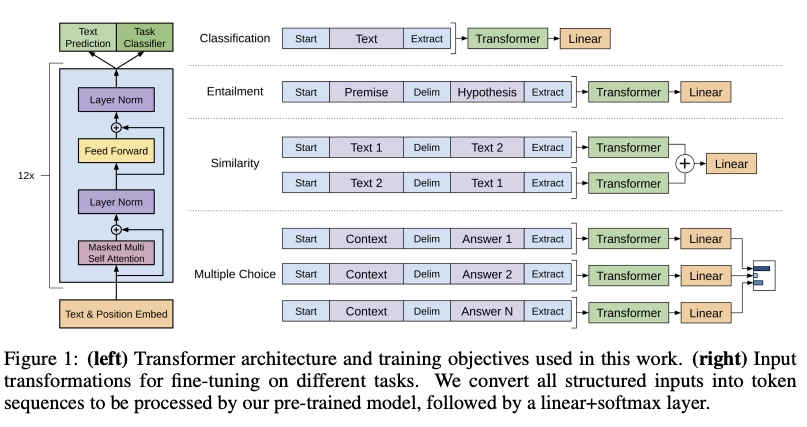
\includegraphics[width=1\linewidth]{img//rnn//transformers/cleanshot-2023-04-16-at-23.39.34.jpeg}
\captionof{figure}{Source: \href{https://s3-us-west-2.amazonaws.com/openai-assets/research-covers/language-unsupervised/language_understanding_paper.pdf}{\textbf{Improving Language Understanding by Generative Pre-Training}})}

\section{Text Generation using pre-trained HuggingFace Transformer
models}\label{text-generation-using-pre-trained-huggingface-transformer-models}

\subsection{Step 1: Load the pre-trained GPT-2
model}\label{step-1-load-the-pre-trained-gpt-2-model}

\begin{lstlisting}[language=Python]
from transformers import GPT2LMHeadModel, GPT2Tokenizer

# Load pre-trained GPT-2 model and tokenizer
model_name = "gpt2"
model = GPT2LMHeadModel.from_pretrained(model_name)
tokenizer = GPT2Tokenizer.from_pretrained(model_name)
\end{lstlisting}

\begin{lstlisting}
/opt/venv/lib/python3.10/site-packages/tqdm/auto.py:21: TqdmWarning: IProgress not found. Please update jupyter and ipywidgets. See https://ipywidgets.readthedocs.io/en/stable/user_install.html
  from .autonotebook import tqdm as notebook_tqdm
\end{lstlisting}

\subsection{Step 2: Define the prompt
text}\label{step-2-define-the-prompt-text}

\begin{lstlisting}[language=Python]
# Define the prompt text
prompt = "The quick brown fox"
\end{lstlisting}

\subsection{Step 3: Generate text using the GPT-2
model}\label{step-3-generate-text-using-the-gpt-2-model}

\begin{lstlisting}[language=Python]
# Generate text using the GPT-2 model
input_ids = tokenizer.encode(prompt, return_tensors="pt")
output = model.generate(input_ids, max_length=50, do_sample=True)

# Decode the generated text
generated_text = tokenizer.decode(output[0], skip_special_tokens=True)
print(generated_text)
\end{lstlisting}

\begin{lstlisting}
The attention mask and the pad token id were not set. As a consequence, you may observe unexpected behavior. Please pass your input's `attention_mask` to obtain reliable results.
Setting `pad_token_id` to `eos_token_id`:50256 for open-end generation.


The quick brown foxes, a new species and then some, are the same from year to year.

That's why some of the latest sightings are often the same.

"We can see all kinds of people, you can hear
\end{lstlisting}

In this example, we used the pre-trained GPT-2 model to generate text
based on a prompt. We first loaded the model and tokenizer using the
Hugging Face Transformers library. Then, we defined the prompt text that
we want the model to generate text from. Finally, we used the
\lstinline{generate()} method to generate text from the
prompt and decode the generated text using the tokenizer. \newline

Note that the \lstinline{generate()} method takes several
arguments, including \lstinline{max_length}, which
controls the maximum length of the generated text, and
\lstinline{do_sample}, which enables sampling from the
model distribution to generate diverse outputs. \newline

This is just a simple example of text generation using the Hugging Face
Transformers library. With this powerful library, you can explore a wide
range of models and tasks in NLP, from language translation to question
answering and beyond. \newline

TODO:

Try
\href{https://huggingface.co/models?pipeline_tag=text-generation&sort=downloads}{other
text generation models} from HuggingFace with different prompts.

\begin{lstlisting}[language=Python]
from transformers import pipeline

generator = pipeline('text-generation', model="facebook/opt-125m")
generator(prompt)
\end{lstlisting}

\begin{lstlisting}
[{'generated_text': "The quick brown fox is a good one.\nI've been using it for a while now."}]
\end{lstlisting}

\section{Text translation using pre-trained
Transformers}\label{text-translation-using-pre-trained-transformers}

\begin{lstlisting}[language=Python]
from transformers import MarianMTModel, MarianTokenizer

model_name = "Helsinki-NLP/opus-mt-en-es"
tokenizer = MarianTokenizer.from_pretrained(model_name)
model = MarianMTModel.from_pretrained(model_name)
\end{lstlisting}

\begin{lstlisting}
/opt/venv/lib/python3.10/site-packages/tqdm/auto.py:21: TqdmWarning: IProgress not found. Please update jupyter and ipywidgets. See https://ipywidgets.readthedocs.io/en/stable/user_install.html
  from .autonotebook import tqdm as notebook_tqdm
/opt/venv/lib/python3.10/site-packages/transformers/models/marian/tokenization_marian.py:194: UserWarning: Recommended: pip install sacremoses.
  warnings.warn("Recommended: pip install sacremoses.")
\end{lstlisting}

First, we import the \lstinline{MarianMTModel} and
\lstinline{MarianTokenizer} classes from the
\lstinline{transformers} module, which is a popular Python
library for working with transformer-based models such as BERT, GPT, and
MarianMT.

Next, we set the \lstinline{model_name} variable to
\lstinline{Helsinki-NLP/opus-mt-en-es}, which is the name
of the pre-trained model that will be used for English-to-Spanish
translation. Read more about this pre-trained model
\href{https://huggingface.co/Helsinki-NLP/opus-mt-en-es}{here}.

The \lstinline{MarianTokenizer} class is then used to
instantiate a \lstinline{tokenizer} object, which will be
used to tokenize the input text before passing it to the model.

Similarly, the \lstinline{MarianMTModel} class is used to
instantiate a translation \lstinline{model} object. The
model object is initialized with the pre-trained weights of the
English-to-Spanish translation model specified by
\lstinline{model_name}.

\begin{lstlisting}[language=Python]
import warnings
warnings.filterwarnings('ignore')

def translate(model, tokenizer, text: str) -> str:
    """
    :param text: English text
    :return: Spanish text (translated from the English input)
    """
    # Tokenize the input text
    inputs = tokenizer(text, return_tensors="pt")
    # Generate the corresponding Spanish translation
    outputs = model.generate(**inputs)
    # Decode the translated text
    translated = tokenizer.decode(outputs[0], skip_special_tokens=True)
    return translated

text = "Hello, how are you doing today?"
translated = translate(model, tokenizer, text)
print(translated)
\end{lstlisting}

TODO:

Try building a text translation application that can detect and
translate text from different languages. You can use the pre-trained
models available
\href{https://huggingface.co/models?pipeline_tag=translation&sort=downloads}{here}.

\section{GPT3 and ChatGPT}

\subsection{GPT-3}

\begin{itemize}
    \item GPT-3 is a language model developed by OpenAI based on transformer architecture.
    \item It was released in June 2020 and is known for its impressive performance on various language tasks.
    \item GPT-3 is trained on over 45 terabytes of text data and has 175 billion parameters.
    \item The model is pre-trained on a language modeling objective, which allows it to learn a general understanding of language, including syntax, semantics, and context.
    \item GPT-3's architecture is based on the transformer, which consists of a stack of transformer layers with multiple attention heads.
    \item The model incorporates several innovations, including relative positional encoding and a mixture of experts to specialize in different areas of language processing.
\end{itemize}
You can use GPT-3 using API developed by OpenAI by creating an account on the \href{https://platform.openai.com/overview}{\textbf{OpenAI website}}. \newline

We also recommend exploring \href{https://platform.openai.com/playground}{\textbf{Open AI playground(opens in a new tab)}} to test GPT-3 and other models for various NLP tasks.

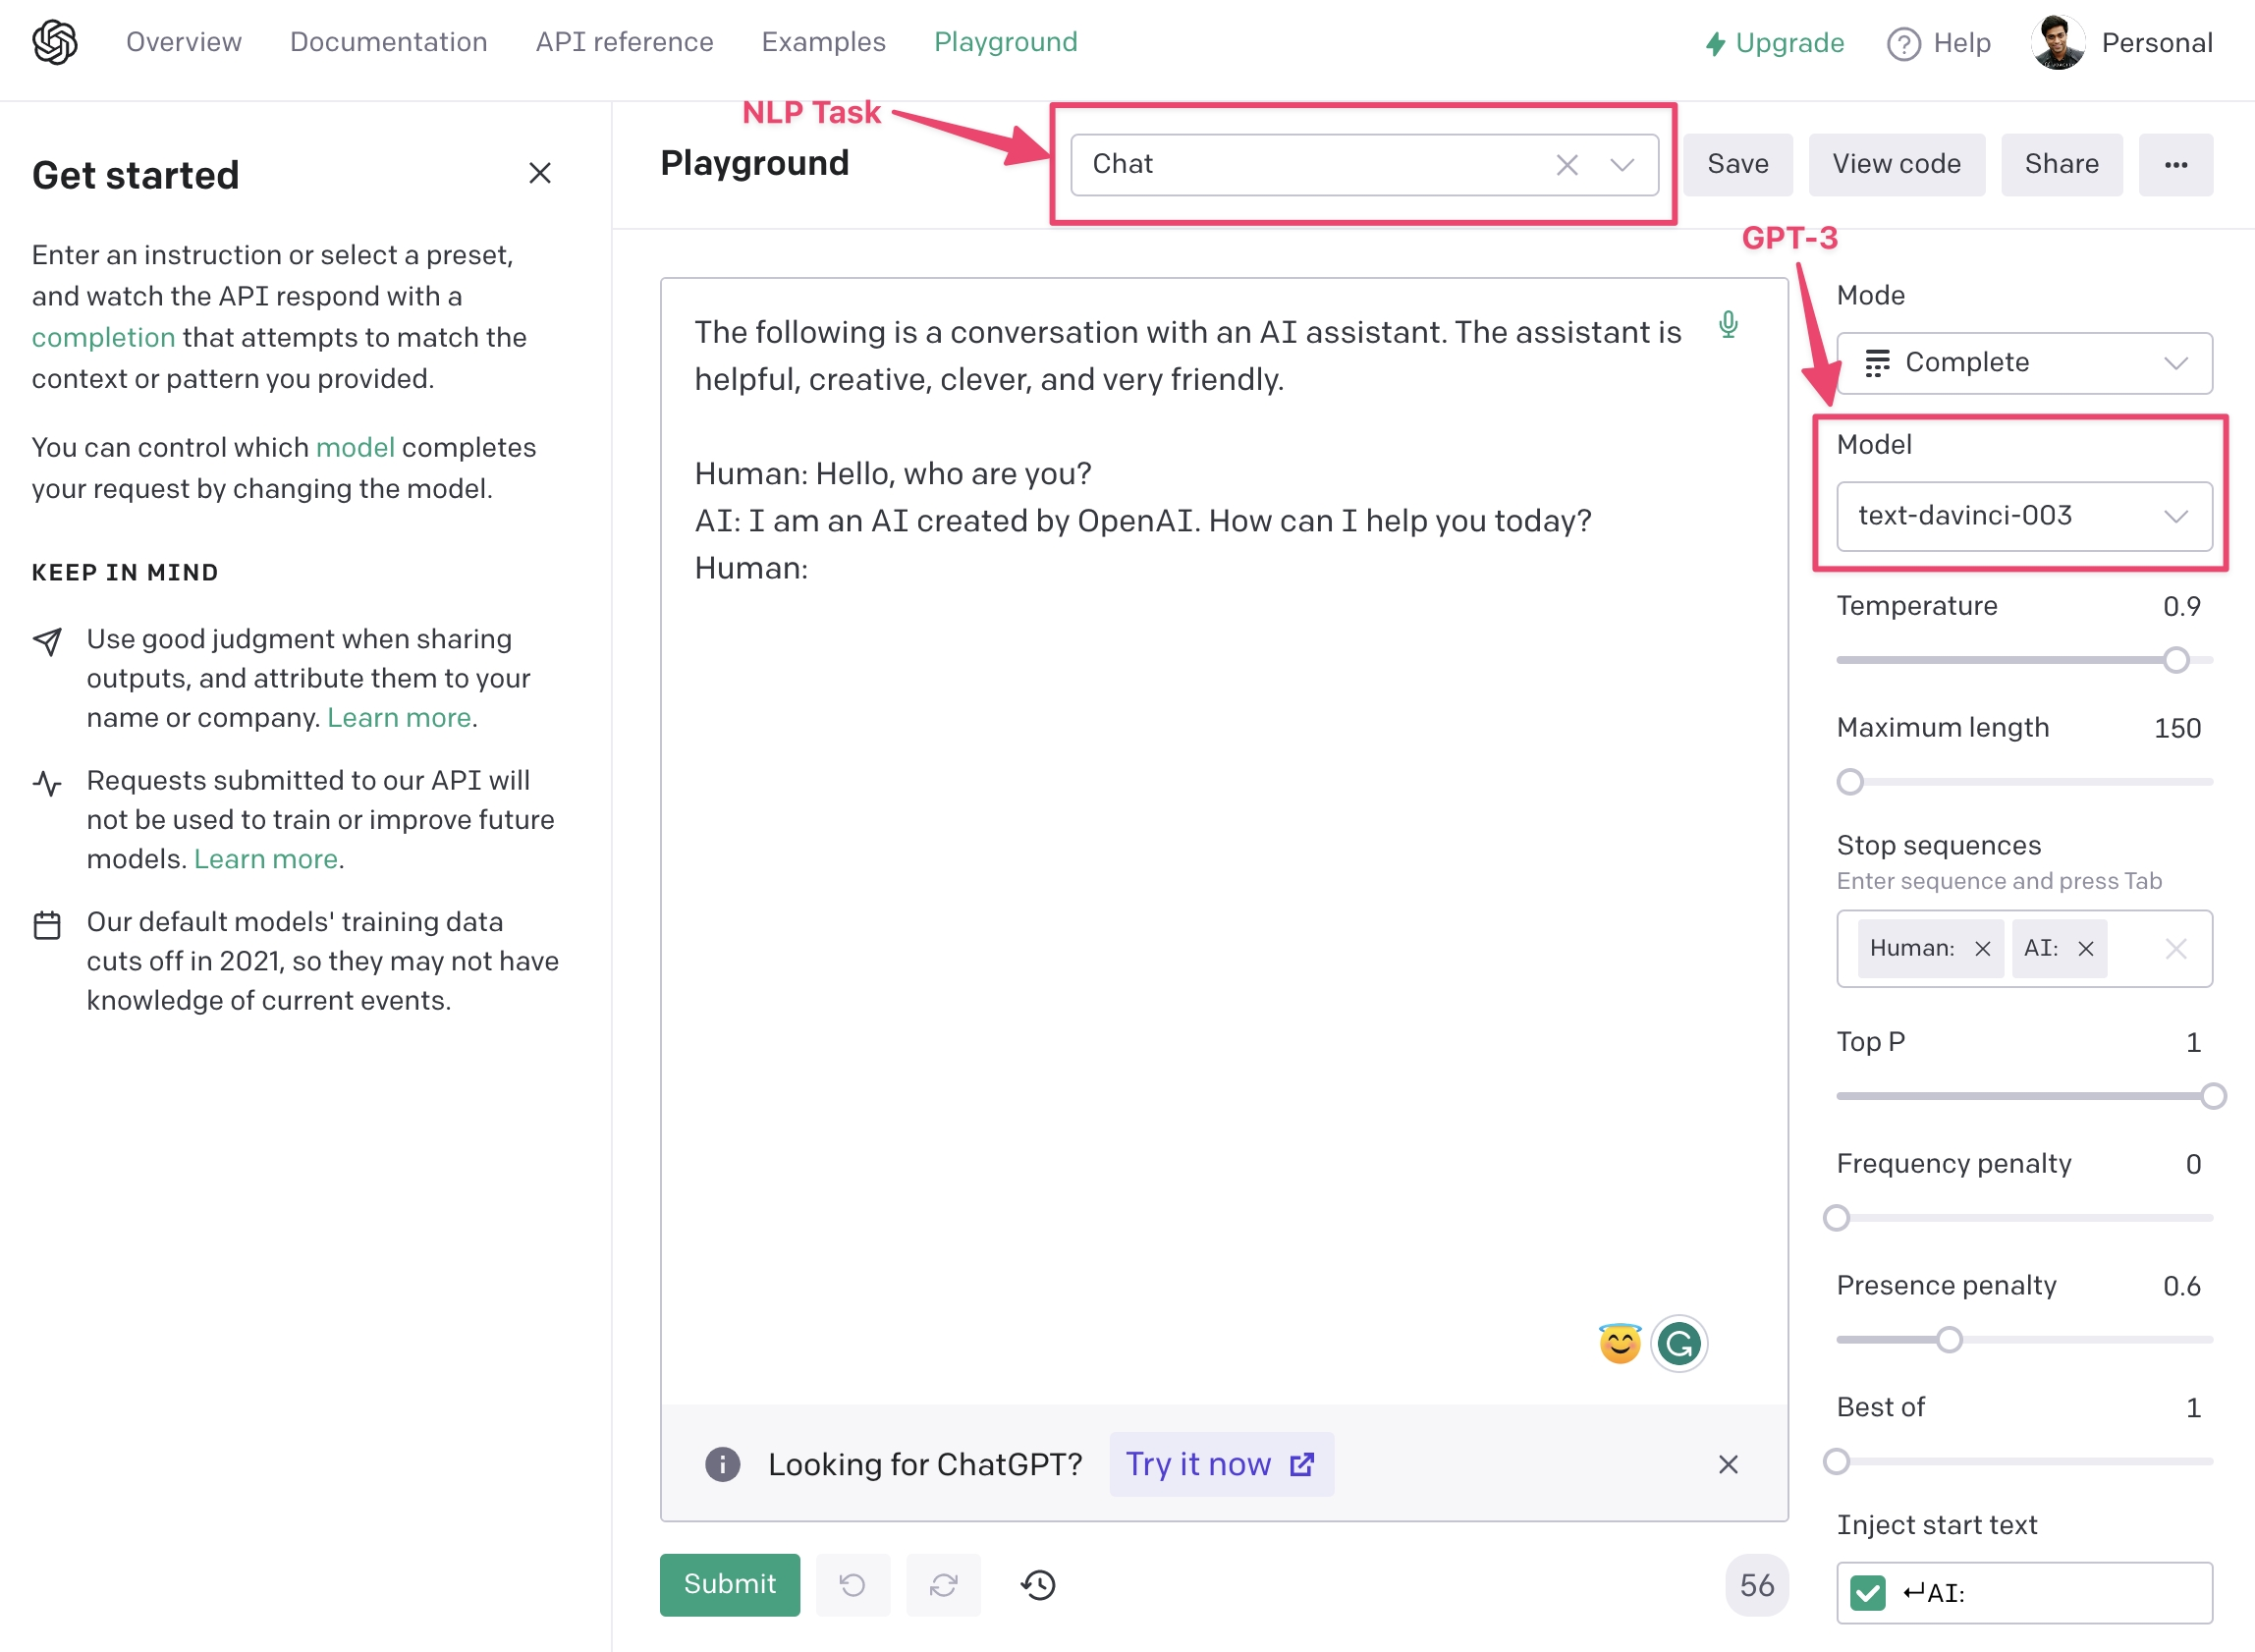
\includegraphics[width=1\linewidth]{img//rnn//transformers/open_ai_playground.jpeg}
\captionof{figure}{Open AI Playground}

Click on \textbf{View Code} if you would like to integrate this model in your application.

\subsection{ChatGPT}

\begin{itemize}
    \item ChatGPT is a large language model developed by OpenAI based on the GPT-4 architecture.
    \item It is an NLP tool that can generate human-like responses to textual input.
    \item ChatGPT has been trained on a vast corpus of text data and can understand the nuances of language, including grammar, syntax, and context.
    \item It can be used for chatbots, customer service, virtual assistants, language learning, tutoring, and more.
    \item ChatGPT has a vast knowledge base and can provide answers to a wide range of questions, making it a valuable resource for researchers, students, and professionals.
    \item Its ability to understand the context of the conversation and generate relevant responses has made it popular for companies looking to automate their customer service and support functions.
    \item ChatGPT's conversational abilities are continuously improving and have the potential to revolutionize the way we interact with machines.
    \item Overall, ChatGPT is a powerful language model with significant potential for various applications, and its capabilities are expected to grow as NLP technology advances.
\end{itemize}
